The concept of implementation can be divided into the used packages (\emph{Stable Baselines3, Gym Pybullet Drones, ...}), the scripts, the environment classes and different support classes (\cref{fig:concept}).\\
Stable Baselines3 is used as implementation of the PPO algorithm (\cref{alg:ppo}) in order to achieve the tasks. Gym Pybullet Drones has already some environments and is the foundation of the simulation. It already provides a suitable step function and a well designed physics engine.\\
The scripts (\cref{sec:scripts} , lila) are used to either learn the agent on a given environment or evaluate it.\\
The environment classes(\cref{sec:env}, green) inherit from a \emph{Gym Environment} and models a MDP. By modelling this MDP precisely, it is defined what is learned later by the intelligent agent. It uses the wind class in order to model a harsh environment.
In addition, there are a couple of evaluation tools (\cref{sec:tools}, red), that supports the implemented classes.\\
\newline
The whole concept is implemented in Python3.x with the use of a \emph{conda environment}.

\begin{figure}[htp]
	\centering
	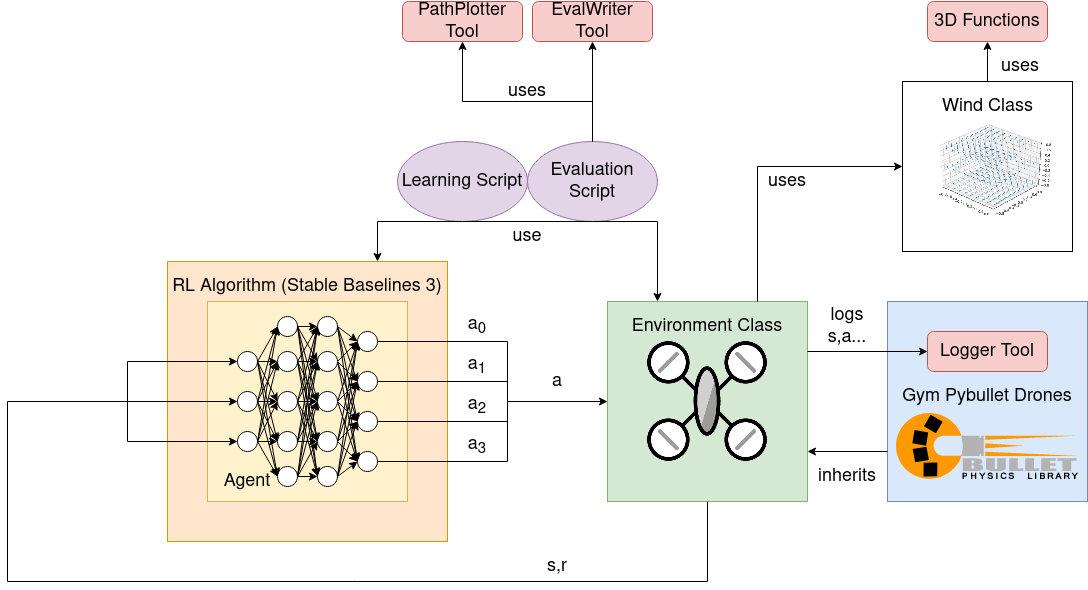
\includegraphics[width= \linewidth]{figures/concept.png}
	\caption{Concept of the implemented software: the different tools(red), scripts(violet) that are used in order to learn the intelligent Agent robust flight control with the use of RL.}
	\label{fig:concept}
\end{figure}
\newpage

\section{Environment Classes} \label{sec:env}



\subsection{WindSingleAgentAviary Environment Class}

\newpage

\subsubsection{Wind Class}

\newpage

\subsubsection{Modes}

\newpage

\subsubsection{State Space}


\subsubsection{Observation Space}

\newpage

\subsubsection{Action Space}
The WindSingleAgentAviary Environment possesses three different type of action spaces, that are processed in different ways to the \emph{rpm (rotation per minute)} of the four motors (\cref{tab:act}). Nevertheless, all action types are continuous and are ranged in $[-1, 1]$.\\
\newline
\emph{one\_d\_rpm} is a one dimensional action space. The chosen action $a$ is processed to range of $\alpha$ about the \emph{hover\_rpm} to a 4-tupel of rpms. The hover\_rpm is defined as the rpm that corresponds to hovering (\cref{sec:hover}). The 4-tupel is then forwarded to the motors. As a consequence of this limitation, the drone can only perform hovering, rising and falling movements and can not influence its $x,y$ position or $\Theta, \phi, \psi$. Also, the translational speed $v_z$ is limited by the size of $\alpha$.\\
\newline
\emph{rpm} is a 4 dimensional action space. The actions are processed within a range of $\alpha$ about the hover\_rpm to a 4-tupel of rpms. The drone is not limited in any dimensionality, but the task increases in complexity. Due to \cref{form:quad}, \cref{form:quad2}, \cref{form:quad3}, \cref{form:quad4} even a small difference in rpms can lead to an unstable flight or even a crash, because the roll or pitch angle is to high. Also, all translational an rotational speeds are limited by the size of $\alpha$. Because of the higher complexity, it is expected, that the training takes noticeable more time.\\
\newline
\emph{vel} is a top level, 4-dimensional action space. The action consists of a velocity vector $v = (a_0, a_1, a_2)$ and its size $a_3$.  Since it is a top level action space, the actions are not corresponding directly to the rpms, but a pid controller (\cref{sec:pid}) is used in order to control the rpms. The basic pid controller is part of Gym Pybullet Drones \cite{panerati2021learning} and must be tuned for the used quadrocopter. It mainly receives the state $S$ of the drone, as well as the targeted velocity, which is calculated with the use of the actions. Therefore, $a_3$ is multiplicated with speed limit of the drone in order to derange the action. Also, the velocity vector $v$ is normalized to a length of $1$.\\
The drone is not limited in any dimensionality and the task is less complex then setting rpm directly. Stability of the flight is now mainly controlled by the pid controller, so it is bounded by the typical pid constraints in harsh environments and not adaptable.
\begin{table}
	\centering
	\caption{The different ActionTypes with the corresponding dimensionality of the action, its range and how it is processed.}\label{tab:act}
	\begin{tabular}{c|c|c|c}
		ActionType & dim & range & processing\\
		\hline
		\emph{one\_d\_rpm} & $|a| = 1$ & $a_i \in [-1, 1]$ & $rpm = (hover\_rpm \cdot (1 + \alpha \cdot  a)) \cdot (1, 1, 1, 1)$ \\
		\emph{rpm} & $|a| = 4$ & $a_i \in [-1, 1]$ & $rpm =  hover\_rpm \cdot (1 + \alpha \cdot  a)$ \\
		\emph{vel} & $|a| = 4$ & $a_i \in [-1,1]$ & $rpm = pid(S, vel= limit \cdot  |a_3| \cdot \frac{(a_0,a_1,a_2)}{|(a_0,a_1,a_2)|})$
	\end{tabular}
\end{table}


\newpage

\subsubsection{Reward}
\begin{figure}
	\centering
	\begin{subfigure}{0.45\linewidth}
		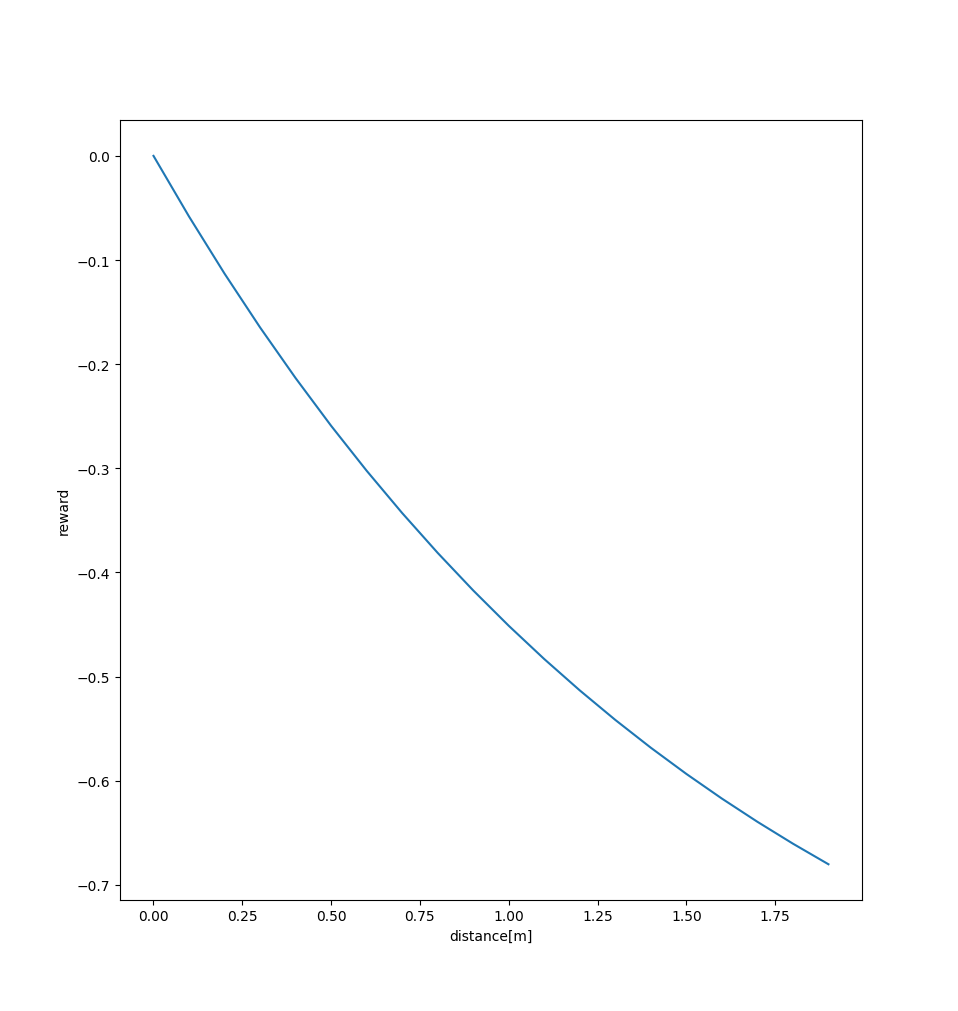
\includegraphics[width=\linewidth]{figures/reward.png}
		\caption{}
	\end{subfigure}
	\begin{subfigure}{0.45\linewidth}
		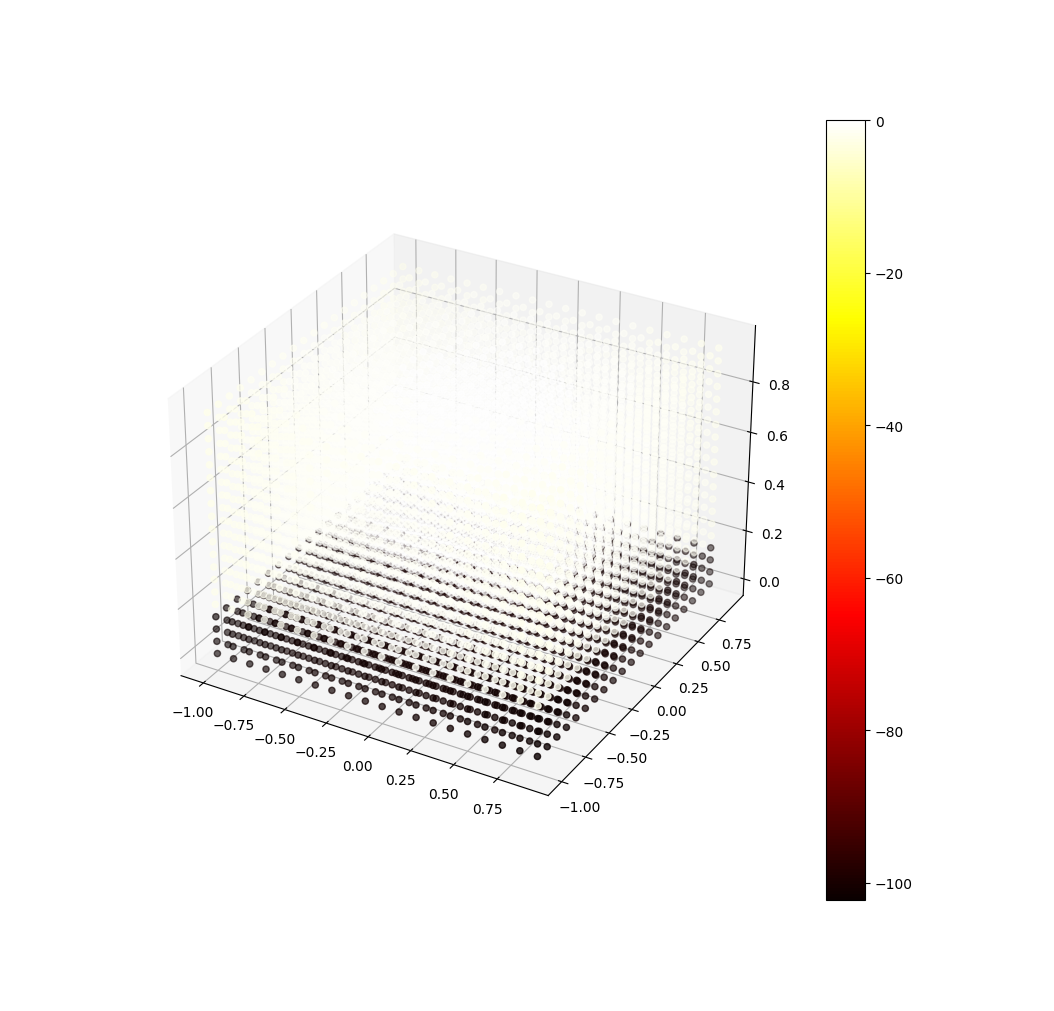
\includegraphics[width=\linewidth]{figures/reward2.png}
		\caption{}
	\end{subfigure}
	\caption{Visualization of the used reward function with the goal ($0,0,0.5$) and a colour scale: the distance dependent part (a) and the big penatalization, because the drone hit the ground (b)}
\end{figure}

\newpage

\subsubsection{Constraints}

\newpage

\subsection{WindSingleAgentPathfollowingAviary Environment Class}


\newpage

%%%%%%%%%%%%%%%%%%%%%%%%%%%%%%%%%%%%%%%%%%%%%
\section{Scripts \& Evaluation Tools} \label{sec:scripts}


%\subsection{TestInstall Script}

\subsection{Learning Script}
\begin{algorithm}
	\caption{Learning Script}
	\label{alg:learn}
	 Parse the arguments to the Script
	 
	 Check the parsed arguments on contradiction and raise ParsingError if needed
	 
	 Create training environment with the parsed parameters
	 
	 Define the size of the actor and critic policy network
	 
	 Create or load the model based on the parsed load argument
	 
	 Create evaluation environment with the parsed parameters
	 
	 Define evaluation callbacks
	 
	 Learn the model with the parsed amount of time steps
	 
	 Save the model with the parsed preferred name
	 
	 
\end{algorithm}

\newpage

\subsection{Evaluation Script}
\begin{algorithm}
	\caption{Evaluation Script}
	\label{alg:eval}
	Parse the arguments to the Script
	
	Check the parsed arguments on contradiction and raise ParsingError if needed
	
	Create evaluation environment with the parsed parameters
	
	Define the size of the actor and critic policy network
	
	Load the model
	
	Instantiate an EvalWriter and evaluate the model
	
	\If{gui parameter was parsed as true}{
		Instantiate a test environement, logger and a pathplotter
		
		Reset environment and safe an observation $\sigma$
		
		
		Safe current time $t$
		
		\Repeat{done or time is over}{
		Get action $a$ and the observation $\sigma$
		
		Execute a step in the test environment and receive an observation $\sigma$, a reward $r$, a done value and a info
		
		Add current pose to pathplotter
		
		Log current drone state
		
		Sync simulation time $t_sim$ to the real time $t$}
		Close test environment, show the plotted path and the values.
	}


\end{algorithm}

\newpage

%%%%%%%%%%%%%%%%%%%%%%%%%%%%%%%%%%%%%%%%%%%%%%
\subsection{Evaluation Tools} \label{sec:tools}

\subsubsection{EvalWriter Class}

\newpage

\subsubsection{PathPlotter Class}
